%%%%%%%%%%%%%%%%%%%%%%%%%%%%%%%%%%%%%%%%%%%%%%%%%%%%%%%%%%%%%%%%%%%%%%%%%%%%%%%%
%2345678901234567890123456789012345678901234567890123456789012345678901234567890
%        1         2         3         4         5         6         7         8

\documentclass[letterpaper, 10 pt, conference]{ieeeconf}  % Comment this line out if you need a4paper

%\documentclass[a4paper, 10pt, conference]{ieeeconf}      % Use this line for a4 paper

\IEEEoverridecommandlockouts                              % This command is only needed if 
                                                          % you want to use the \thanks command

\overrideIEEEmargins                                      % Needed to meet printer requirements.

% See the \addtolength command later in the file to balance the column lengths
% on the last page of the document

% The following packages can be found on http:\\www.ctan.org
\usepackage{cite}
\usepackage{graphicx} % for pdf, bitmapped graphics files
%\usepackage{epsfig} % for postscript graphics files
%\usepackage{mathptmx} % assumes new font selection scheme installed
%\usepackage{times} % assumes new font selection scheme installed
%\usepackage{amsmath} % assumes amsmath package installed
%\usepackage{amssymb}  % assumes amsmath package installed

\title{\LARGE \bf
CoffeeBot
}


\author{Jason Rebello$^{1}$ and Ian Colwell$^{2}$% <-this % stops a space
%\thanks{*This work was not supported by any organization}% <-this % stops a space
%\thanks{$^{1}$Albert Author is with Faculty of Electrical Engineering, Mathematics and Computer Science,
%        University of Twente, 7500 AE Enschede, The Netherlands
%        {\tt\small albert.author@papercept.net}}%
%\thanks{$^{2}$Bernard D. Researcheris with the Department of Electrical Engineering, Wright State University,
%        Dayton, OH 45435, USA
%        {\tt\small b.d.researcher@ieee.org}}%
}


\begin{document}


\maketitle
\thispagestyle{empty}
\pagestyle{empty}


%%%%%%%%%%%%%%%%%%%%%%%%%%%%%%%%%%%%%%%%%%%%%%%%%%%%%%%%%%%%%%%%%%%%%%%%%%%%%%%%
\begin{abstract}

Robotics holds tremendous potential for benefiting every domain of human life. Over the years, the focus of robotics has shifted from the design of a mechanical structure with the integration of electronics that can perform a small set of predefined tasks to complex machines capable of operating intelligently in everyday scenarios. This process is highly involved and requires the understanding of several key concepts in order to make it truly autonomous. In this paper we will address the main ideas such as mapping, localization and navigation for a coffee delivery unmanned ground vehicle (UGV) in an office setting. We will present a comparison of two path planners (PRM and Astar) in terms of their run-time, path generated and total distance travelled to reach a desired location.

\end{abstract}

%%%%%%%%%%%%%%%%%%%%%%%%%%%%%%%%%%%%%%%%%%%%%%%%%%%%%%%%%%%%%%%%%%%%%%%%%%%%%%%%
\section{INTRODUCTION/MOTIVATION}

There is a growing need for robots to operate intelligently and adapt to their changing environment without direct human supervision. The delivery chain is one of the main areas where autonomous robots have established a foothold.
One of the most important tasks that nurses in a hospital spend a lot of time doing is giving medications to patients. Hospitals move an immense amount of materials through hallways, on elevators, in basements and to patient units. This is a complex demanding internal logistics challenge that has implications of cost, quality and safety. Automating delivery of this material generates considerable savings and efficiency. It usually requires a human to make a dedicated trip to a pharmacy that may be on a different floor of the hospital. This sort of thing is a waste of time for highly trained medical professionals, which is why a robot makes sense to have as a delivery system. 
In this paper we will present our method at developing an autonomous robot for coffee delivery to a particular room on the third floor of engineering 5. Although the project was undertaken with the task of coffee delivery the concepts employed can be used for any other autonomous delivery system as stated above. One of the significant challenges in developing an autonomous robot is its ability to effectively localize itself in a predefined map while navigating to a specific location. We will present our approach at tackling these problems and perform a comparison of our custom Probabilistic roadmap and A-star path planning techniques in terms of optimal path generation, runtime to generate paths and ways of improvement. 
The rest of the paper is organized as follows. In section 2, we present an overview of the various companies developing autonomous robots for industry. Section 3, describes the hardware and software used in our setup. Section 4 explains our methodology used in our project which includes the navigation stack. Section 5 discusses our custom path planners and performs a comparison of the two methods. Section 6 concludes our work and states methods for improvement and future work.

\section{BACKGROUND WORK}

There are a host of companies that have started developing autonomous robots for industrial tasks such as manufacturing and delivery of goods.? Amazon? has undertaken the development of autonomous drones as part of its Prime Air delivery system. ?Google? has recently announced its desire to deliver packages from self-driving trucks. ?Clearpath Robotics? specializes in the design and manufacture of unmanned vehicle solutions for industrial and academic applications. ?Autonomous Solutions Inc? has provided unmanned vehicle hardware and software systems to clients in mining, industrial and military markets. More aligned with our project is the ?Tug? autonomous medical robot from ?Aethon? that delivers and transports medicines in an efficient and safe manner. Similarly, ?Panasonic? has been working on its ?Hospi? hospital delivery robot in order to ferry small and important objects and materials from one place to another. In most of these robots, the main sensors are some form of Lidar sensor (mostly 3D) that give fast response and at the same time provide good field of view. Due to its light weight, a camera is used as a primary tool for place recognition during localization.

\section{SYSTEM OVERVIEW}

\subsection{Hardware Used} 

We use the Husky unmanned ground vehicle manufactured by Clearpath Robotics as our mobile robotic platform. The Husky is a four wheeled skid steer system built for both outdoor and indoor use. The advantage of using the husky is its large payload capacity and power systems that can accommodate a variety of sensors. We make use of the UTM-30LX laser scanner by Hokuyo. One of the main advantages of using this sensor is its high accuracy and angular resolution. The sensor returns a list of range measurements in the form of a 2D point cloud. This sensor is extremely useful in doing scan registration for mapping and localization. The final sensor used is the Microsoft Xbox Kinect sensor. The Kinect contains a color VGA video camera which is used to take RGB images and an infrared depth sensor that returns a 3D point cloud that aligns with the RGB image to form a complete RGB-D image. A wireless Logitech handheld controller was also used for test driving the coffeebot. A laptop was used as the main controller for the coffeebot. All communications to and from the laptop were over USB ports. The complete hardware setup is shown in Figure \ref{hardware}. 

	\begin{figure}[!ht]
		\centering
		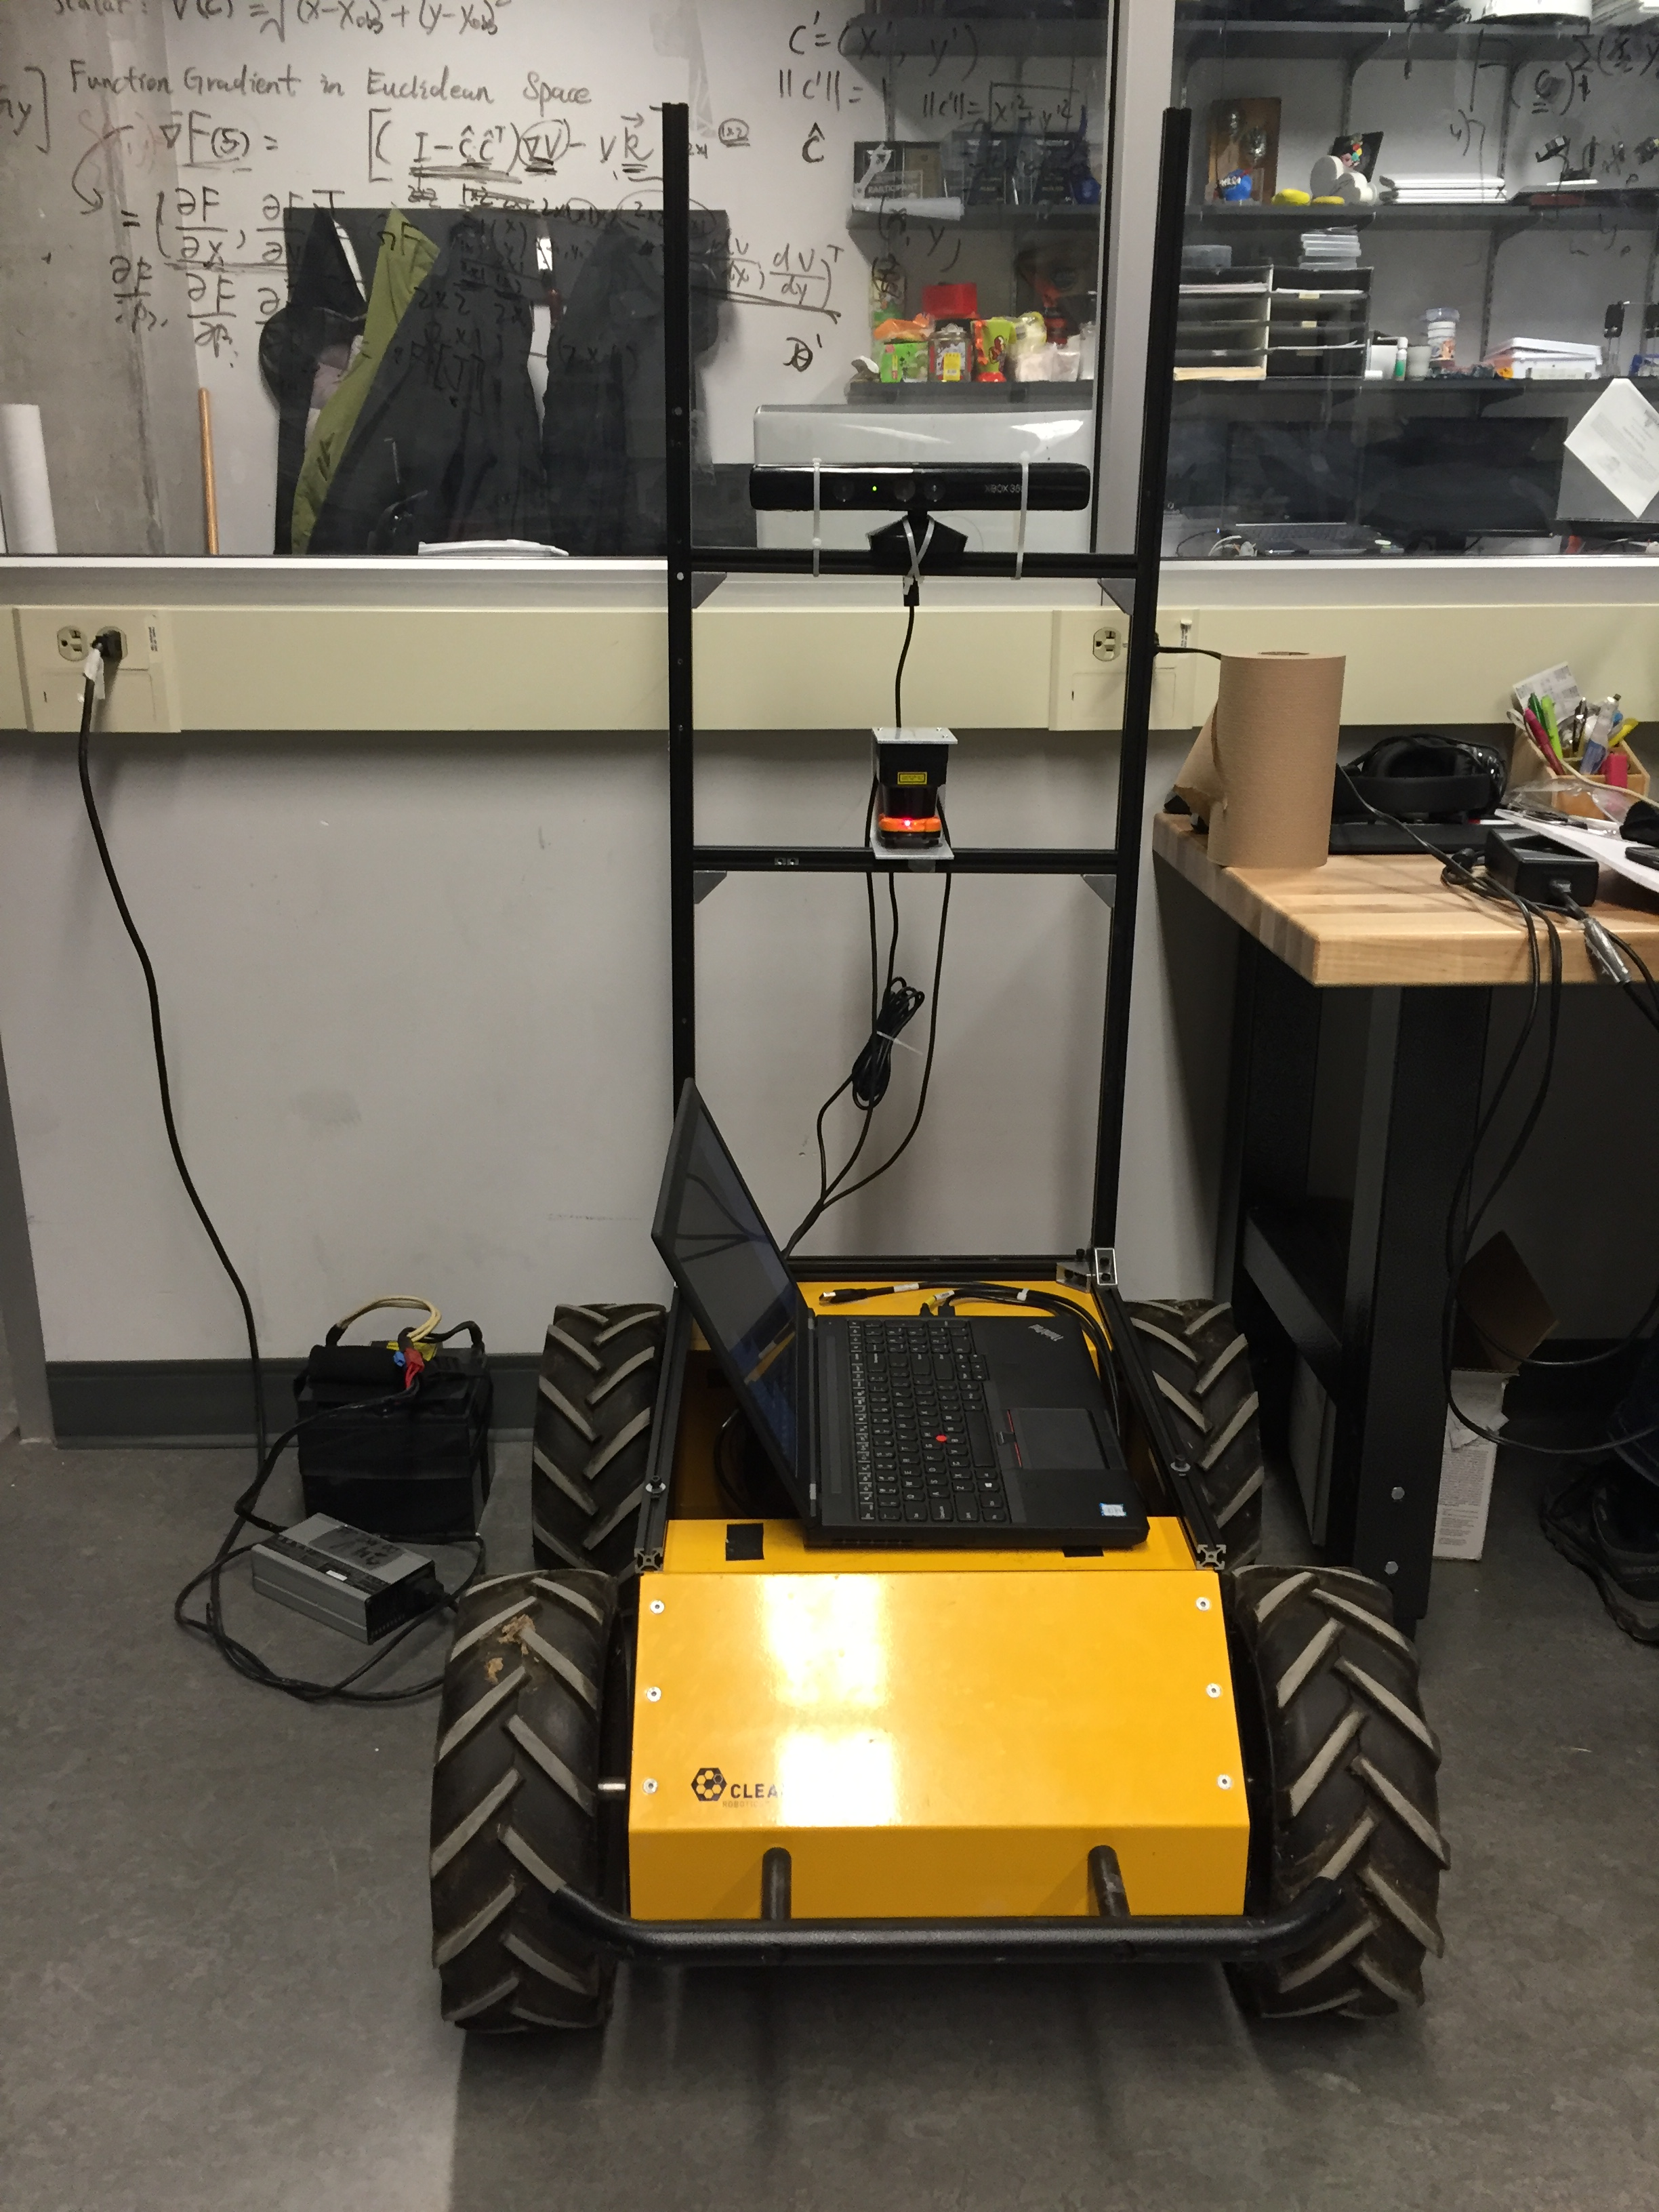
\includegraphics[width=1.0\columnwidth]{Figures/hardware_setup}
		\caption{The coffeebot.}
		\label{hardware}
	\end{figure}

\subsection{Software Used}

The software framework used for this project was ROS (Robot Operating System). ROS provided a convenient framework to build the coffeebot system using both existing open source ROS packages and the newly created coffeebot ROS package. The most important ROS packages used are briefly mentioned below, more detail will be provided in the corresponding section that utilizes the packages. The system architecture is then described after the package descriptions.

\subsubsection{RTAB-Map}

RTAB-Map is used for mapping the environment and then localizing within it. RTAB-Map stands for "Real-Time Appearance-Based Mapping" and is a RGB-D Graph-Based SLAM approach based on an incremental appearance-based loop closure detector~\cite{rtabmap2014}.
This project used rtabmap for two main functions. First, mapping was performed of the environment in which the robot will be operated. RTAB-Map is capable of generating both a 3D point cloud map and also a 2D occupancy grid that is aligned with the point cloud. The map generated by RTAB-Map also contains a graph based image library. Feature extraction is used on the image library for loop closure detection. Second, localization within the generated map was another core function provided by RTAB-Map. The localization function allowed the robot to be located within the previously built occupancy grid which is essential for path planning.

\subsubsection{ROS Navigation Stack}

The ROS navigation stack is a set of ROS packages designed for moving a robot autonomously. The stack primarily consists of cost map generation for obstacle avoidance and path planning/execution for moving the robot. The 'move\_base' ROS node was used to tie all the navigation stack functions together and issue commands to drive the robot. 

\subsubsection{Coffeebot}

A new ROS package was created for the coffeebot project which consisted of three main parts. Each part will be covered in more detail in the corresponding section of this report. The first important part of the package is the launch files. Launch files were created to run the coffeebot, run husky simulations, and build maps from previously recorded data. Second, a ROS service was created to issue navigation goals based on room number requests. Third, a global path planner was written as a plugin to the navigation stack. 

\subsubsection{RViz}

Finally, RViz was used to visualize all the data being passed around inside ROS. RViz is a popular data visualization tool that is easy to configure. Custom configurations were created specifically for the coffeebot in order to make debugging quicker and easier. 

The various pieces of software came together to create a functional system as shown in Figure . Figure XX is a simplified system architecture describing the system while in navigation mode. Figure XX shows the relevant transforms of the system. When the coffeebot is in navigation mode, the RTAB-Map ROS node is receiving input from the laser scanner, kinect, and the odometry measurements from the Husky. RTAB-Map uses this data to estimate a position of the coffeebot relative to the predefined map. Once the first successful feature match (loop closure) is detected then RTAB-Map publishes the occupancy grid and localizes the robot within the map. Once the occupancy grid is published, the navigation stack subscribes to it and creates the global cost map. Assuming the occupancy grid is not updated, the global cost map is only generated once and remains static throughout the operation session. The navigation stack also creates a local costmap that is updated four times a second using data from the Kinect and laser scanner. The local costmap is constructed using both laser scanner and kinect data which allows the robot to avoid obstacles that do not appear in the plane of the laser scanner. 
Global paths can be created once the global cost map is available to the navigation stack. A global path is generated using a global path planner and only takes into account the global cost map. Once the global path is generated through the global costmap, a local planner generates trajectories through the local costmap that track the global path. If there is poor alignment between the local and global costmaps, the local planning may fail or get stuck. Finally, the local trajectories are then sent directly to the 'husky\_base' ROS node to be executed by the husky. 

	\begin{figure}[!ht]
		\centering
		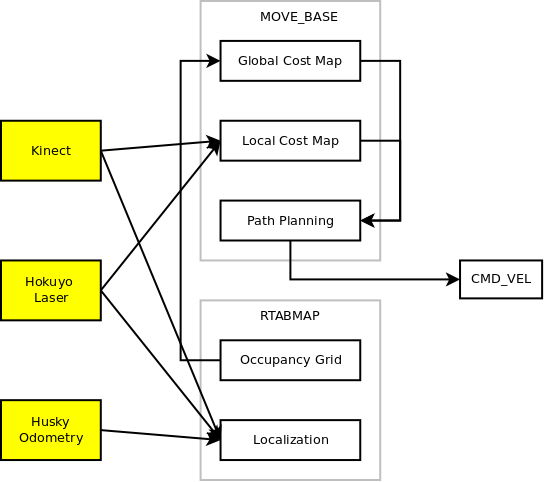
\includegraphics[width=1.0\columnwidth]{Figures/ROS_node_diagram}
		\caption{The simplified software architecture of the coffeebot.}
		\label{software_architecture}
	\end{figure}
	
	\begin{figure}[!ht]
		\centering
		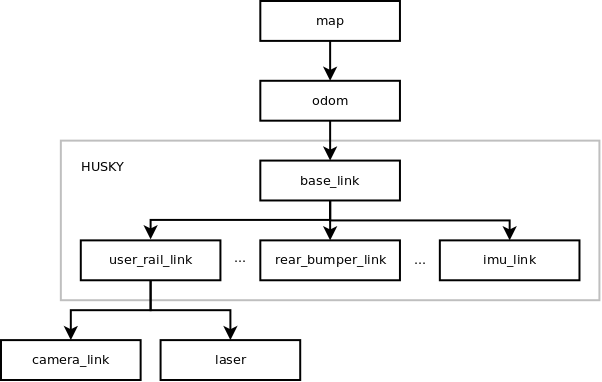
\includegraphics[width=1.0\columnwidth]{Figures/ROS_TF_diagram}
		\caption{The transforms of the coffeebot.}
		\label{transform_tree}
	\end{figure}

\section{Methodology}

\subsection{Mapping}

Autonomous robots operating in real life settings must be able to navigate in large, unstructured, dynamic and unknown spaces. To do so they must build a map of their operating environment. A map of the 3rd floor of Engineering 5 was built with the help of RTabmap as described in Section 3 while utilizing g2o and vertigo. The ?generalized graph optimization? (g2o) framework is an open-source C++ framework for optimizing graph-based nonlinear error functions. Vertigo is a C++ extension that enables g2o to solve pose graph SLAM problems in 2D and 3D despite a large number of false positive loop closure constraints. RTabmap mainly relies on the detection of SURF features in order extract visual words from the scene. Since the robot is constrained to operate in a single plane, the transformation can be refined with 2D iterative-closest-point (ICP) optimization using laser scans. With the help of ICP an occupancy grid map is generated. This grid map will then be used to generate the static global cost map during path planning.

*** 1) Map of whole floor 2) zoomed in version of hallway 3) Occupancy grid *****

\subsection{Localization}

Once a map of the environment is completed, it is essential to be able to localize the robot within the existing map each time the robot is restarted. Without localization, the previously generated map is useless for navigation purposes. Fortunately, RTAB-Map includes a localization mode that works very similar to the mapping mode. In localization mode, feature matches are detected (Figure \ref{localization}) between the saved image library and the input from the RGB-D camera (kinect). If sufficient matching is found then an estimate is made on the position of the robot within the map. This is very similar to the loop closure detection performed in mapping mode, the only difference being that no new constraints are added to the graph. Once the first successful feature match (loop closure) is detected then RTAB-Map publishes the occupancy grid and updates the 'map' transform which locates the robot within the map relative to the starting location of the robot ('odom' transform) as shown in Figure

	\begin{figure}[!ht]
		\centering
		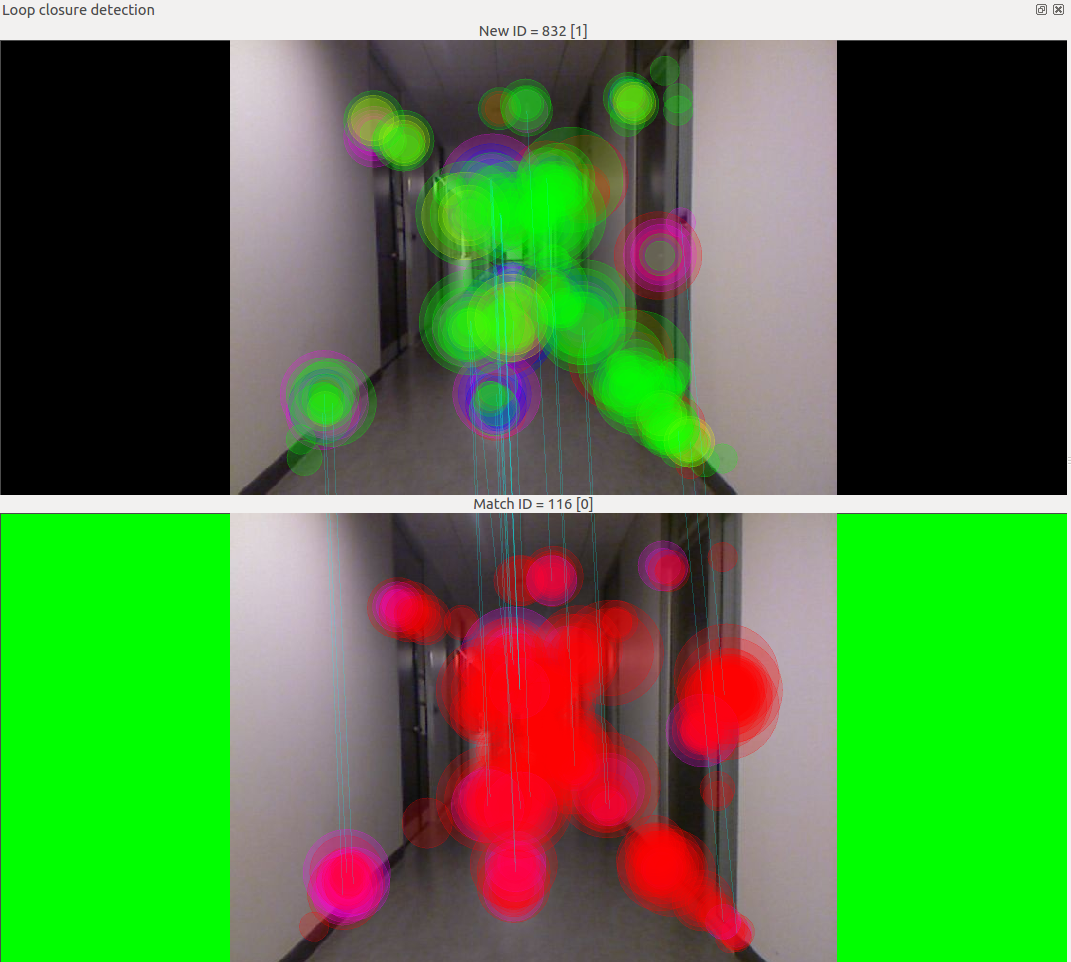
\includegraphics[width=1.0\columnwidth]{Figures/loop_closure}
		\caption{A successful feature based loop closure.}
		\label{localization}
	\end{figure}

	\begin{figure}[!ht]
		\centering
		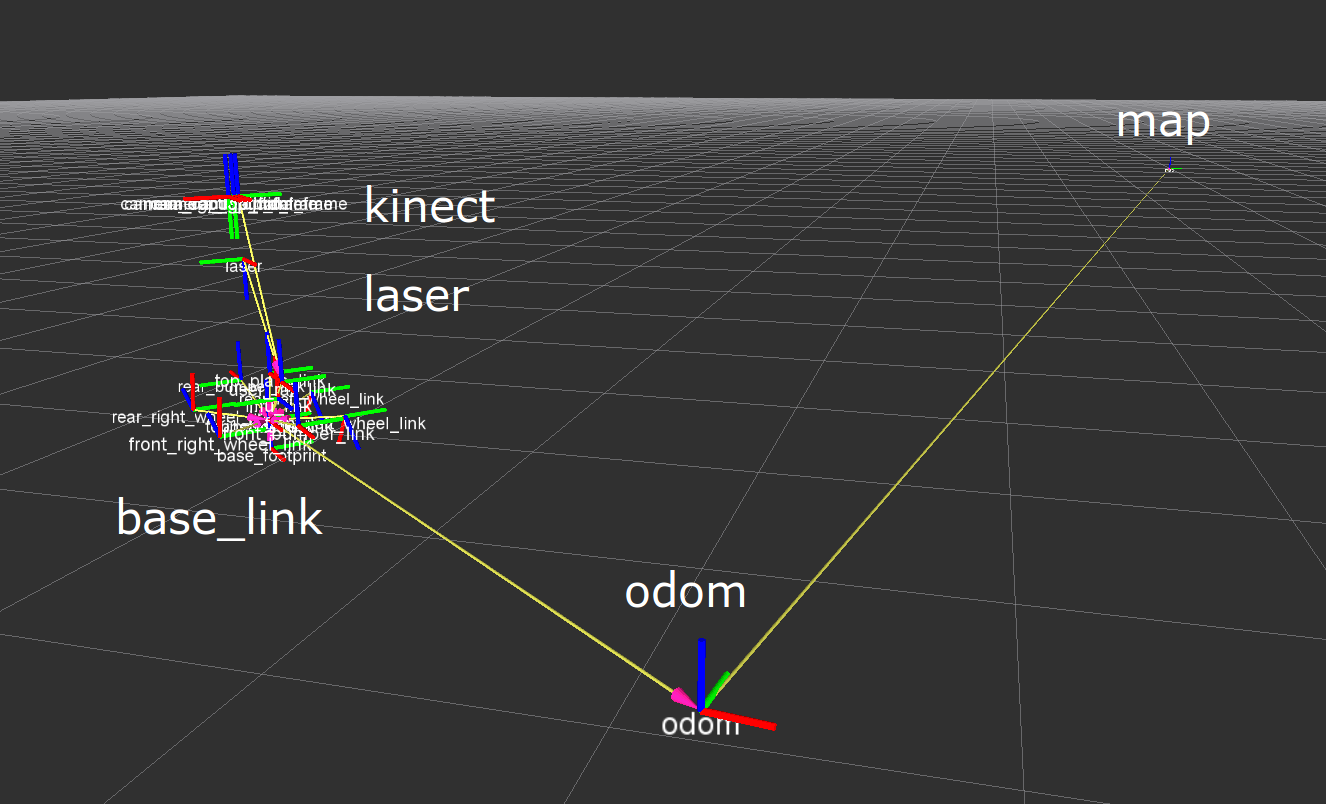
\includegraphics[width=1.0\columnwidth]{Figures/Transforms}
		\caption{The Coffeebot transforms with respect to odom and map.}
		\label{transforms}
	\end{figure}

\subsection{Planning/Navigation}

The navigation stack was used for path planning and navigation of the Coffeebot. The stack mainly consists of both a local and global costmap and a both a local and global path planner. The global costmap is generated from the predefined occupancy grid and the local costmap is generated live based on sensor data. A small ROS service was also created that issues goal locations based on room number requests. The service simply runs in a terminal and only takes one request at a time. As part of the navigation to various rooms, two global path planning algorithms were developed and compared. Both planners were created as global planner plugins to the ROS navigation stack for easy integration with ROS.

\subsubsection{Costmaps}
The local costmap is limited in size and is centered around the robot. This ensures dynamic objects seen in the past are not saved when returning to the area the object was first detected. Both local and global costmaps are generated using a decaying cost inflation technique. This technique assigns the highest cost to detected objects then assigns gradually lower costs out to the specified inflation radius where a cost of zero is assigned which represents free space. The 2D planar size of the robot is called the ?footprint? and is considered when building the costmaps. The dimensions used for the husky is 1 meter long and 0.65 meters wide. In Figure \ref{global_costmap} below, yellow represents an occupied cell in the occupancy grid, Aqua represents a location where the robot is definitely in collision (based on the robot footprint), Red represents a location where the robot may be in collision depending on the orientation of the robot, and Blue represents a buffer zone to keep the robot away from obstacles.

	\begin{figure}[!ht]
		\centering
		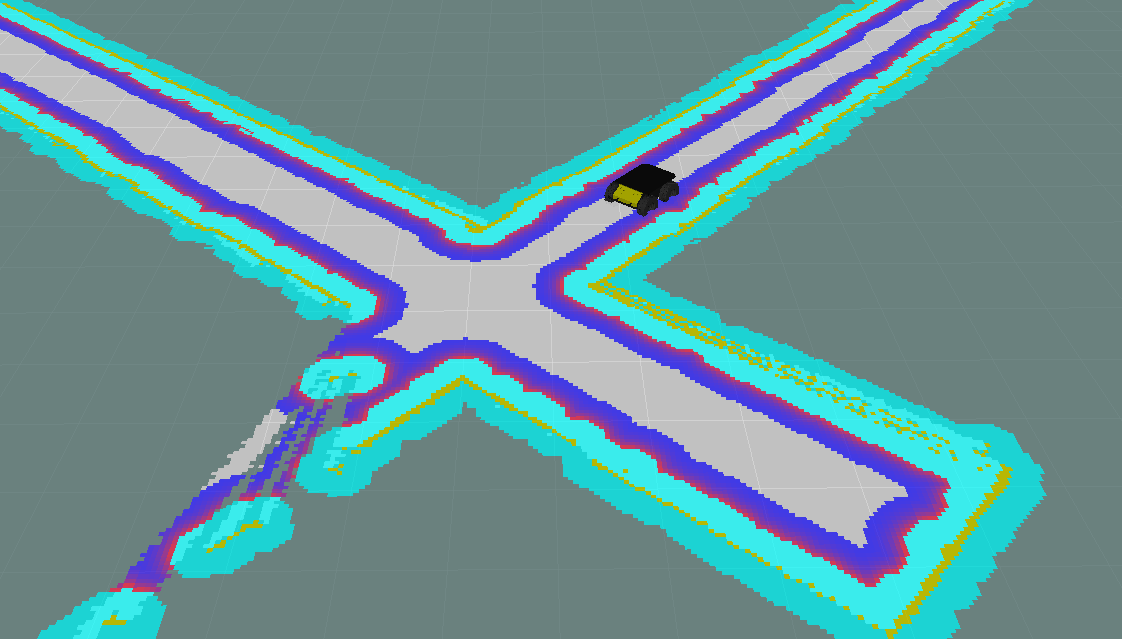
\includegraphics[width=1.0\columnwidth]{Figures/global_costmap}
		\caption{The global costmap with costs shown in colour.}
		\label{global_costmap}
	\end{figure}

\subsection{Global PRM Planner}

A custom global planner was created to generate paths for the coffeebot. The planner utilized a global costmap provided by the navigation stack to find paths between start and goal locations while avoiding areas of cost. The Probabilistic Roadmap (PRM) technique was utilized to generate a path. Creating a Probabilistic Road Maps starts with randomly sampling either the configuration space of the robot or the physical environment of the robot. While the Husky is non-holonomic, it is able to turn on the spot. For this reason, and to avoid unnecessary over complication, it was decided to sample over the environment space instead of the configuration space. Each random sample consisted of a world coordinate on the global cost map (both an X and Y position in meters). As each sample is created, the corresponding cell of the costmap is checked for a cost. If the cost is less than the allowable cost threshold then the sample is added to a list of milestones. The start and goal locations are also added as milestones if they are located in cells below the cost threshold. The completed milestone list is then iterated over to find the 20 nearest milestones to each milestone. A line to each of the nearest milestones is traced over the costmap using the bresenham line algorithm. While the line is being traced, each costmap cell in the line is checked to determine if the cost of the cell is greater than the cost threshold. The lines between milestones that can be traced without passing over costly cells are then added as edges in the roadmap (red lines in Figure \ref{PRM_planner}). Once all the available edges are created a graph based A-Star search algorithm is employed to find the shortest path through the network. The final step of the path generation is path refinement. The path returned by A-Star is then refined by attempting to skip nodes in the graph. Starting from the goal node and working back, the same bresenham line cost checking as mentioned earlier is used to check the line, or 'shortcut', between the goal node and the third-from-last node. If this line is found to be clear of costs then the second-from-last node is dropped from the path. This process repeats until every 'shortcut' in the path results in traversing a cell of cost.
Finally, the refined path (green line in Figure \ref{PRM_planner}) is sent back to the move\_base node in the form of geometry\_msgs type ROS messages to be tracked by the local planner. For debugging purposes, the network is also published using visualization\_msgs type ROS messages for easy display in RViz. 

	\begin{figure}[!ht]
		\centering
		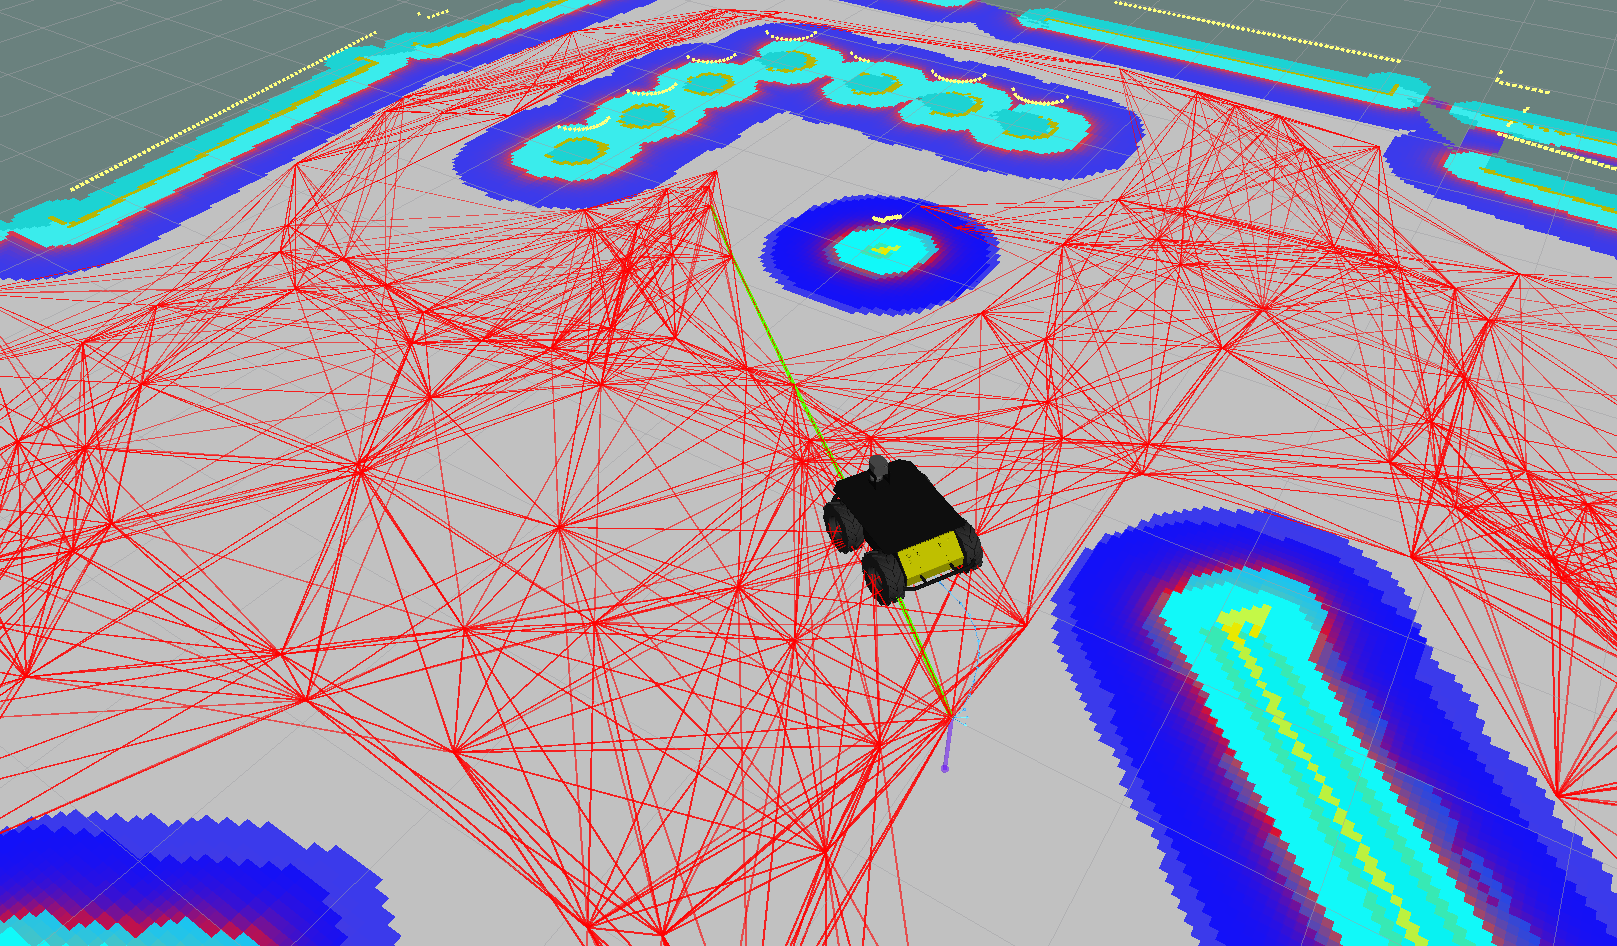
\includegraphics[width=1.0\columnwidth]{Figures/PRM_CloseUP}
		\caption{The PRM planner as seen in RViz.}
		\label{PRM_planner}
	\end{figure}

\subsection{A-Star Global Planner}

The A* algorithm combines features of uniform-cost search and pure heuristic search to efficiently compute optimal solutions. A* algorithm is a best-first search algorithm in which the cost associated with a node is f(n) = g(n) + h(n), where g(n) is the cost of the path from the initial state to node n and h(n) is the heuristic estimate or the cost of the path from node n to the goal. Thus, f(n) estimates the lowest total cost of any solution path going through node n. At each point a node with lowest f value is chosen for expansion. Ties are broken randomly. The algorithm terminates when a goal is chosen for expansion. A* algorithm guides an optimal path to a goal if the heuristic function h(n) is admissible, meaning it never over-estimates the actual cost. 

\section{RESULTS}

\subsection{Mapping and Localization}

A map of the third floor of Engineering 5 was completed. This map includes a 2D occupancy grid as well as an RTAB-Map database which consists of a 3D point cloud and graph based image library. The resulting occupancy grid is shown below in Figure \ref{third_occ_grid} and a portion of the 3D point cloud is shown in Figure \ref{third_point_cloud}.

	\begin{figure}[!ht]
		\centering
		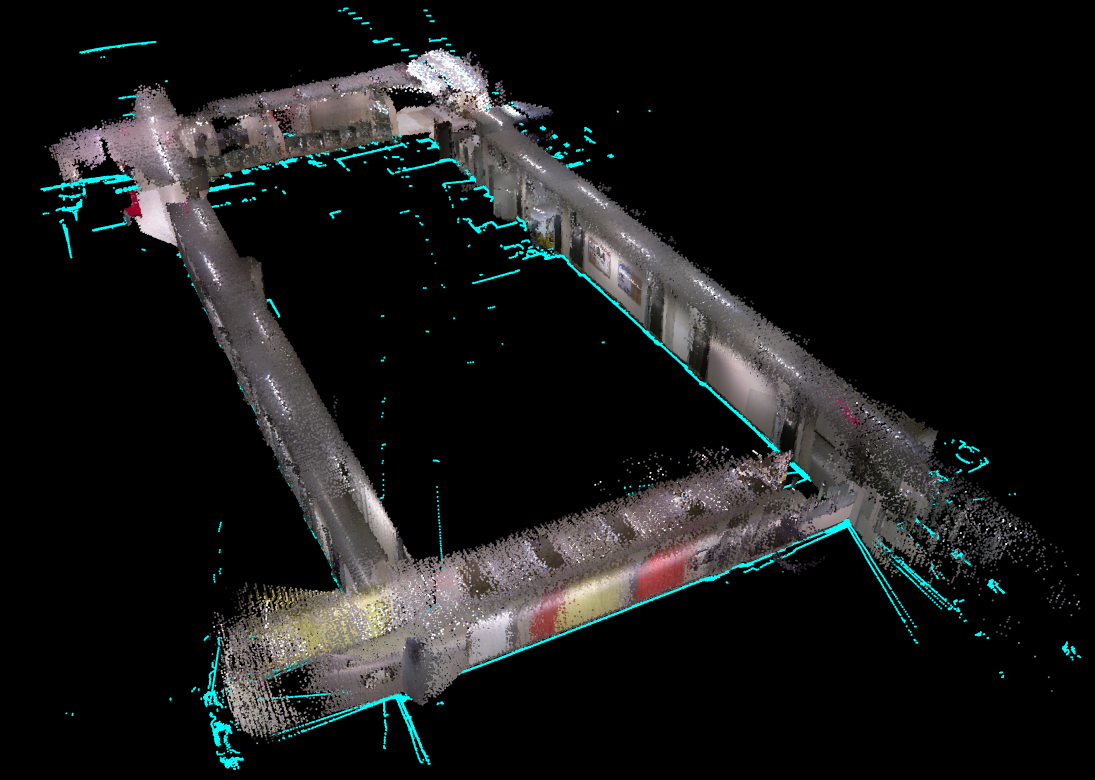
\includegraphics[width=1.0\columnwidth]{Figures/3rdfloor_point_cloud}
		\caption{The 3D point cloud map of the third floor of E5.}
		\label{third_point_cloud}
	\end{figure}
	
	\begin{figure}[!ht]
		\centering
		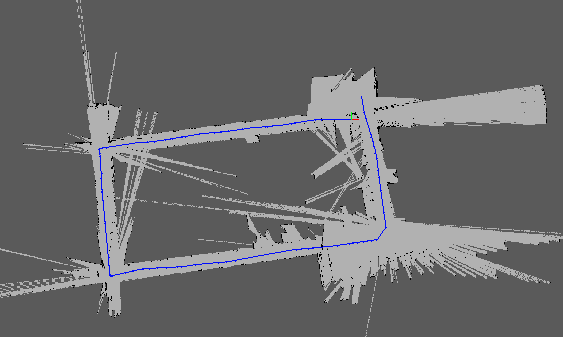
\includegraphics[width=1.0\columnwidth]{Figures/3rd_occupancy_grid}
		\caption{The occupancy grid map of the third floor of E5.}
		\label{third_occ_grid}
	\end{figure}

The coffeebot was also able to successfully localize within the map as shown in Figure XX.

\begin{table}[h]
\caption{An Example of a Table}
\label{table_example}
\begin{center}
\begin{tabular}{|c||c|}
\hline
One & Two\\
\hline
Three & Four\\
\hline
\end{tabular}
\end{center}
\end{table}

\section{CONCLUSION AND FUTURE WORK}

In the future there will be a need for teams of small, agile autonomous robotic units to perform intelligence, surveillance and reconnaissance (ISR) missions. As a result, we would like to extend the coffeebot to communicate with quadrotors. Person following and tracking is another area of interest. In industry most robots are programmed to perform specific tasks. However if the robot can track a ?master? it will have the ability to learn new tasks.


\section{CONCLUSIONS}

A conclusion section is not required. Although a conclusion may review the main points of the paper, do not replicate the abstract as the conclusion. A conclusion might elaborate on the importance of the work or suggest applications and extensions. 

\addtolength{\textheight}{-12cm}   % This command serves to balance the column lengths
                                  % on the last page of the document manually. It shortens
                                  % the textheight of the last page by a suitable amount.
                                  % This command does not take effect until the next page
                                  % so it should come on the page before the last. Make
                                  % sure that you do not shorten the textheight too much.

%%%%%%%%%%%%%%%%%%%%%%%%%%%%%%%%%%%%%%%%%%%%%%%%%%%%%%%%%%%%%%%%%%%%%%%%%%%%%%%%


%%%%%%%%%%%%%%%%%%%%%%%%%%%%%%%%%%%%%%%%%%%%%%%%%%%%%%%%%%%%%%%%%%%%%%%%%%%%%%%%


%%%%%%%%%%%%%%%%%%%%%%%%%%%%%%%%%%%%%%%%%%%%%%%%%%%%%%%%%%%%%%%%%%%%%%%%%%%%%%%%
\section*{APPENDIX}

Appendixes should appear before the acknowledgment.

\section*{ACKNOWLEDGMENT}

blah blah

%%%%%%%%%%%%%%%%%%%%%%%%%%%%%%%%%%%%%%%%%%%%%%%%%%%%%%%%%%%%%%%%%%%%%%%%%%%%%%%%

\bibliographystyle{Bibliography/IEEEtran}

\bibliography{Bibliography/coffeebot}





\end{document}